\documentclass{article}
\usepackage{tikz}
\usetikzlibrary{decorations.markings}
\usepackage{amsmath}
\usepackage{amsfonts}

\DeclareMathOperator{\HH}{H}
\DeclareMathOperator{\Hom}{Hom}
\DeclareMathOperator{\Gal}{Gal}
\DeclareMathOperator{\GL}{GL}
\DeclareMathOperator{\PGL}{PGL}
\DeclareMathOperator{\PGSp}{PGSp}
\DeclareMathOperator{\Res}{Res}


\newcommand{\HT}[1]{\widehat{\HH}^{#1}}
\newcommand{\T}{\mathbf{T}}
\newcommand{\Th}{\hat{\T}}
\newcommand{\CC}{\mathbb{C}}

\title{Rectifiers}
\author{Moshe Adrian and David Roe}
\date{\today}

\begin{document}
\maketitle

\section{Questions}

\begin{enumerate}
\item Prove that the character $\chi$ of the coinvariants that Gross gives you, agrees with the cohomology class $c_L$ of the group of type $L$, when restricted to $\HT{-1}$.

We wrote down the following diagram.

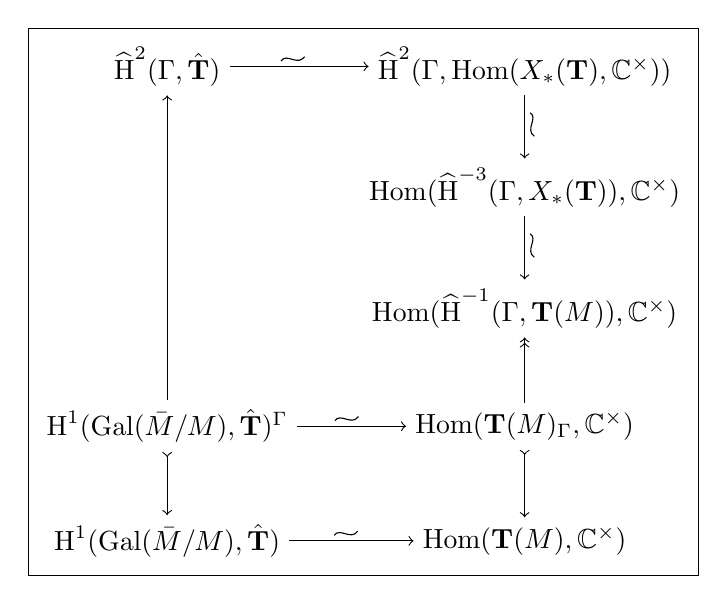
\begin{tikzpicture}[iso/.style={postaction={decorate,decoration={markings, mark=at position 0.45 with {\draw [-] (-4pt,2pt) .. controls (-2pt,5pt) and (2pt, 0pt) .. (4.5pt, 3.5pt);}}}}]
\matrix [draw,nodes=draw,row sep=8mm,column sep=8mm,every node/.style={line width=0pt}]
{
  \node (n00) {$\HT{2}(\Gamma, \Th)$}; & \node (n01) {$\HT{2}(\Gamma, \Hom(X_*(\T), \CC^\times))$}; \\
  & \node (n11) {$\Hom(\HT{-3}(\Gamma, X_*(\T)), \CC^\times)$}; \\
  & \node (n21) {$\Hom(\HT{-1}(\Gamma, \T(M)), \CC^\times)$}; \\
  \node (n30) {$\HH^1(\Gal(\bar{M}/M), \Th)^{\Gamma}$}; & \node (n31) {$\Hom(\T(M)_{\Gamma}, \CC^\times)$}; \\
  \node (n40) {$\HH^1(\Gal(\bar{M}/M), \Th)$}; & \node (n41) {$\Hom(\T(M), \CC^\times$)}; \\
};
\draw [->, iso] (n00) to (n01);
\draw [->, iso] (n01) to (n11);
\draw [->, iso] (n11) to (n21);
\draw [->>] (n31) to (n21);
\draw [>->] (n31) to (n41);
\draw [->, iso] (n30) to (n31);
\draw [->, iso] (n40) to (n41);
\draw [>->] (n30) to (n40);
\draw [->] (n30) to (n00);
\end{tikzpicture}

The arrow $\HH^1(\Gal(\bar{M}/M), \Th)^{\Gamma} \rightarrow \HH^2(\Gamma, \Th)$ fits into the inflation-restriction sequence
\begin{multline*}
0 \rightarrow \HH^1(\Gamma, \Th) \rightarrow \HH^1(\Gal(\bar{M}/K), \Th) \rightarrow \\
 \HH^1(\Gal(\bar{M}/M), \Th)^\Gamma \rightarrow \HH^2(\Gamma, \Th) \rightarrow \HH^2(\Gal(\bar{M}/K), \Th).
 \end{multline*}

So if we want the diagram to commute then we would hope that $\HH^2(\Gal(\bar{M}/K), \Th)$ would vanish....

\item We have defined a base point Langlands parameter that we want to give the correct rectifier.  What difference does it make to send Frobenius to the Tits group element than to any other lift of the Weyl group element defining the group of type $L$?  Answer : We figured out that it doesn't matter if $G$ is semisimple.  But if $G = \GL_2$, then it does matter, we can't just pick any lift.  We have to pick Tits group element (up to a sign?)

\item Let $w$ be an elliptic element of a Weyl group.  Let $\sigma_w$ be the Tits group lift.  Under what conditions is the order of $w$ equal to the order of $\sigma_w$?  This would say that the group of type $L$ splits.  But more generally, under what conditions is there a lift of $w$ that has the same order of $w$?  This would also say that the group of type $L$ splits, so we don't just want to look at the Tits group lift.  We just want to ask when can we lift $w$ to an element in the normalizer that has the same order as $w$. (right?)

\item Check that our conjectural rectifier agrees with the rectifiers for $\PGL_2(F)$, $\PGSp_4(F)$, $\GL_n(F)$, $\PGL_n(F)$ and for all semisimple groups in the DeBacker/Reeder setup.  Partial Answer: We already checked that if $G$ is semisimple, we get the correct rectifier in the DeBacker/Reeder setup. We also checked that we get the same rectifier for $\GL_n(F)$ where $n$ is prime, if the Langlands parameter is tame.

\item Can we use the central character to help us in the case that $\HT{0}$ is nontrivial?  That is, Gross's groups of type $L$ gives us a character on the image of the norm map, which is a subgroup of $T(F)$.  So we don't get a full character of $T(F)$ from Gross's groups of type $L$.  But can we combine what we do get, with a conjectural central character, to get a full character of $T(F)$?

\item In a case outside of DeBacker/Reeder, do we get various expected properties of $L$-packets?

\item What about $\GL_2(F)$, in the ramified situation?  Can we get the rectifier naturally here?  That would be great if we could.

\item Sending Frobenius to the Tits group element is natural because sending to other choices of lifts of the Weyl group element give you the wrong rectifier.

\item Our rectifier agrees with $\GL_n(F)$ in the tame case and $n$ prime.  Does it agree with $\GL_n(F)$ in the tame case where $n$ is arbitrary?  That would be really great.  Start with $\GL_4(F)$, then move on to $\GL_6(F)$ maybe.

\item I have a write-up of various results about tori, unramified in particular.  In the notes $\HT{-1}$ and $\HT{0}$ are calculated in general, for compact unramified tori.  I know you have calculated $\HT{0}$ in your thesis, but I didn't see $\HT{-1}$.  I have a very nice write-up of both of this stuff, and I think we should include it in our paper.

\item Suppose that $w \in W$ is an element of the Weyl group of order $n$, and suppose that $\sigma(w)$ is the Tits group element lifting $w$.  Then
$$\sigma(w)^n = \exp\left(\pi i \sum_{j=0}^{n-1} w^j \cdot \rho^\vee\right),$$
where $\rho^{\vee}$ is half the sum of positive roots.

\item The Langlands parameter that gives you the rectifier on $T(E)_{\Gamma}$ should be the Langlands parameter that gives you the trivial character of $T(F)$ if you run this Langlands parameter through the DeBacker/Reeder theory (to get a character of $T(F)$).

\item Jeff Adams mentioned to me that it would be nice if we could prove that if $\phi_1, \phi_2$ are Langlands parameters, and if they are both associated to the same torus $T(F)$, then the rectifiers associated to $\phi_1, \phi_2$ are equal.  (But I think after all is said and done, this will be obvious.  It sort of already is, since all that matters is where Frobenius goes in order to determine the rectifier.  So yes, if you have two Langlands parameters for $T(F)$, the rectifiers are the same...i.e. the Langlands parameters can be different on inertia.  This really is just a remark that should go in our paper.  It's nothing deep.)

\item Here is a relevant conjecture that Jeff Adams and I came up with as we were sitting down together one time: Let $w$ be any Weyl group element, and let $\sigma(w)$ be a canonical Tits group lift.  Suppose $w^n = 1$.  Then $$\sigma(w)^n = e^{\pi i(\rho^{\vee} - w \rho^{\vee} - w^2 \rho^{\vee} - ... - w^{n-1} \rho^{\vee})}$$  I have some notes on our discussion about this, in particular, notes on trying to prove this conjecture.  My notes are where my ``Contragredient'' binder/notes are.

\item To prove that $\hat{H}^0(\Gamma, T(E)) = 0$ for $T$ a torus that comes from the DeBacker/Reeder paper, maybe use that any torus equals a multipliciative product of its maximal split subtorus and its maximal split anisotropic torus???

\item Question : Should rectifiers for classical groups be compatible with rectifiers for $GL(n)$? ie functoriality, lifting, etc.?

\item To figure out the Langlands parameter associated to rectifiers for $E/F$ ramified for $GL(2,F)$, try to see if JK Yu's local Langlands for tori will tell me what the Langlands parameter is, if I know the rectifier


\end{enumerate}

\section{Outline}

\begin{enumerate}
\item Introduction and summary (Gross's work, Bushnell-Henniart)
\item Cohomology of tori (from Moshe and Gordan, David works on ramified tori)
\item Our definition of rectifier
\item Check that our definition is compatible with previous work
\begin{enumerate}
\item Debacker-Reeder (semisimple and maybe in general)
\item Bushnell-Henniart ($\GL_n$)
\end{enumerate}

\end{enumerate}

\section{Notes}

\begin{enumerate}
\item Can we use $R^\times$ instead of $R^*$?
\item How is Gross' construction related to mine?
\item Numbering in sections
\item Be clearer about the difference between $T_0$ and $T(o_E)$
\item We'll probably want to revise Section 9 once we know exactly what we need from DeBacker and Reeder.  In particular, we should mention the fact that $\chi_\phi$ is obtained via the local Langlands correspondence.
\item  Restructure so that our construction comes first and a later section is devoted to compatibility with Reeder-DeBacker
\end{enumerate}

\subsection{Langlands' version of torus correspondence}

$K$ is the splitting field of $T$.

$K^\times \rightarrow W_{K/F}$, where $K^\times$ is playing the role of $W_K$.
\begin{align*}
H^1(W_F, \hat{T}) &\cong H^1(W_{K/F}, \hat{T}) \\
&\cong \Hom(H_1(W_{K/F}, X_*(T)), \CC^\times) \\
&\cong \Hom(H_1(K^\times, X_*(T))^{\Gal(K/F)}, \CC^\times) \\
&\cong \Hom(T(F), \CC^\times)
\end{align*}

What are these isomorphisms?  Note that $\hat{L}$ in Langlands' paper is our $X_*(T)$ and $C_K$ is our $K^\times$.
\begin{enumerate}
\item $H^1(W_{K/F}, \hat{T}) \cong \Hom(H_1(W_{K/F}, X_*(T)), \CC^\times)$ is described at the bottom of page 11 of Langlands' paper.
\item $H_1(W_{K/F}, X_*(T)) \cong H_1(K^\times, X_*(T))^{\Gal(K/F)}$ is $\Res$ at the bottom of page 3: this map is injective and the image is the Galois invariants.  Proving this statement takes a while.
\item $H_1(K^\times, X_*(T))^{\Gal(K/F)} \cong T(F)$ is the middle of page 3.
\end{enumerate}

\end{document}